\chapter{Verkkojen perusteet}

Voimme ratkaista monia algoritmisia ongelmia
esittämällä tilanteen \emph{verkkona} ja käyttämällä sitten
sopivaa verkkoalgoritmia.
Tyypillinen esimerkki verkosta on tieverkosto,
joka muodostuu kaupungeista ja niiden välisistä teistä.
Tällaisessa verkossa ongelmana voi olla selvittää vaikkapa,
kuinka voimme matkustaa kaupungista $a$ kaupunkiin $b$.

Tässä luvussa aloitamme verkkoihin tutustumisen
käymällä läpi verkkojen käsitteitä sekä tapoja
esittää verkkoja ohjelmoinnissa.
Tämän jälkeen näemme, miten voimme tutkia verkkojen rakennetta
ja ominaisuuksia syvyyshaun ja leveyshaun avulla.
Seuraavissa kirjan luvuissa jatkamme verkkojen käsittelyä ja
opimme lisää verkkoalgoritmeja.

\section{Verkkojen käsitteitä}

Verkko muodostuu \emph{solmuista} ja
niitä yhdistävistä \emph{kaarista}.
Merkitsemme verkon solmujen
määrää kirjaimella $n$ ja kaarten määrää
kirjaimella $m$.
Lisäksi numeroimme verkon solmut kokonaisluvuin
$1,2,\dots,n$.
Esimerkiksi kuvassa \ref{fig:veresi} on verkko,
jossa on 5 solmua ja 7 kaarta.

\begin{figure}
\center
\begin{center}
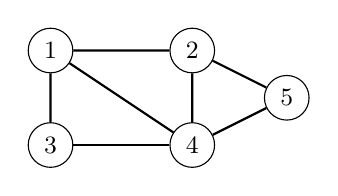
\begin{tikzpicture}[scale=0.6]
\small
\node[draw, circle] (1) at (1,3) {$1$};
\node[draw, circle] (2) at (4,3) {$2$};
\node[draw, circle] (3) at (1,1) {$3$};
\node[draw, circle] (4) at (4,1) {$4$};
\node[draw, circle] (5) at (6,2) {$5$};

\path[draw,thick,-] (1) -- (2);
\path[draw,thick,-] (1) -- (3);
\path[draw,thick,-] (1) -- (4);
\path[draw,thick,-] (3) -- (4);
\path[draw,thick,-] (2) -- (4);
\path[draw,thick,-] (2) -- (5);
\path[draw,thick,-] (4) -- (5);
\end{tikzpicture}
\end{center}
\caption{Verkko, jossa on 5 solmua ja 7 kaarta.}
\label{fig:veresi}
\end{figure}

Sanomme, että kaksi solmua ovat \emph{vierekkäin} verkossa,
jos niiden välillä on kaari.
Solmun \emph{naapureja} ovat kaikki solmut,
joihin se on yhteydessä kaarella,
ja solmun \emph{aste} on sen naapureiden määrä.
Verkossa oleva \emph{polku} tarkoittaa reittiä
tietystä solmusta toiseen kulkemalla kaaria pitkin.
Kuvassa \ref{fig:veresi} solmun 2 naapurit ovat 1, 4 ja 5,
joten solmun aste on 3.
Voimme kulkea solmusta 1 solmuun 5
esimerkiksi polkua $1 \rightarrow 2 \rightarrow 5$
tai $1 \rightarrow 3 \rightarrow 4 \rightarrow 5$.

Sanomme, että verkko on \emph{yhtenäinen},
jos minkä tahansa kahden solmun välillä on polku.
Kuvan \ref{fig:veresi} verkko on yhtenäinen,
mutta kuvan \ref{fig:veryht} verkko ei ole yhtenäinen,
koska esimerkiksi solmujen $1$ ja $2$ välillä ei ole polkua.
Voimme esittää verkon aina kokoelmana yhtenäisiä \emph{komponentteja}.
Esimerkiksi kuvassa \ref{fig:veryht} yhtenäiset komponentit
ovat $\{1,3\}$ ja $\{2,4,5\}$.

\begin{figure}
\center
\begin{center}
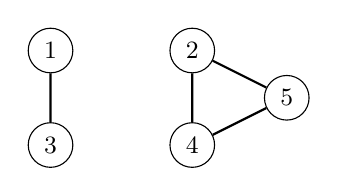
\begin{tikzpicture}[scale=0.6]
\small
\node[draw, circle] (1) at (1,3) {$1$};
\node[draw, circle] (2) at (4,3) {$2$};
\node[draw, circle] (3) at (1,1) {$3$};
\node[draw, circle] (4) at (4,1) {$4$};
\node[draw, circle] (5) at (6,2) {$5$};

\path[draw,thick,-] (1) -- (3);
\path[draw,thick,-] (2) -- (4);
\path[draw,thick,-] (2) -- (5);
\path[draw,thick,-] (4) -- (5);
\end{tikzpicture}
\end{center}
\caption{Verkon yhtenäiset komponentit ovat $\{1,3\}$ ja $\{2,4,5\}$.}
\label{fig:veryht}
\end{figure}

Verkossa oleva \emph{sykli} on polku,
jonka alku- ja loppusolmu on sama,
mutta jokainen muu solmu esiintyy polulla vain kerran.
Kuvan \ref{fig:veresi} verkossa on esimerkiksi
syklit $1 \rightarrow 3 \rightarrow 4 \rightarrow 2 \rightarrow 1$
ja $2 \rightarrow 4 \rightarrow 5 \rightarrow 2$.
Jos verkossa ei ole syklejä, sanomme,
että se on \emph{syklitön}.

\begin{figure}
\center
\begin{center}
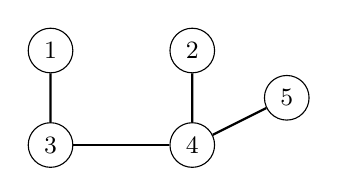
\begin{tikzpicture}[scale=0.6]
\small
\node[draw, circle] (1) at (1,3) {$1$};
\node[draw, circle] (2) at (4,3) {$2$};
\node[draw, circle] (3) at (1,1) {$3$};
\node[draw, circle] (4) at (4,1) {$4$};
\node[draw, circle] (5) at (6,2) {$5$};

\path[draw,thick,-] (1) -- (3);
\path[draw,thick,-] (3) -- (4);
\path[draw,thick,-] (2) -- (4);
\path[draw,thick,-] (4) -- (5);
\end{tikzpicture}
\end{center}
\caption{Yhtenäinen, syklitön verkko eli puu.}
\label{fig:veresi}
\end{figure}

Jos verkko on sekä yhtenäinen että syklitön,
kutsumme sitä nimellä \emph{puu}.
Tällaisessa verkossa jokaisen kahden solmun
välillä on yksikäsitteinen polku.
Jos poistamme minkä tahansa kaaren puusta,
se ei ole enää yhtenäinen,
ja jos lisäämme minkä tahansa kaaren,
puuhun tulee sykli.

\subsection{Suunnatut verkot}

\begin{figure}
\center
\begin{center}
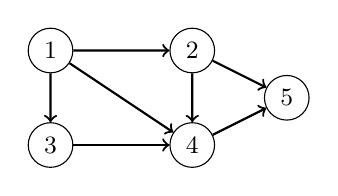
\begin{tikzpicture}[scale=0.6]
\small
\node[draw, circle] (1) at (1,3) {$1$};
\node[draw, circle] (2) at (4,3) {$2$};
\node[draw, circle] (3) at (1,1) {$3$};
\node[draw, circle] (4) at (4,1) {$4$};
\node[draw, circle] (5) at (6,2) {$5$};

\path[draw,thick,->] (1) -- (2);
\path[draw,thick,->] (1) -- (3);
\path[draw,thick,->] (1) -- (4);
\path[draw,thick,->] (3) -- (4);
\path[draw,thick,->] (2) -- (4);
\path[draw,thick,->] (2) -- (5);
\path[draw,thick,->] (4) -- (5);
\end{tikzpicture}
\end{center}
\caption{Suunnattu verkko.}
\label{fig:veresi}
\end{figure}

\subsection{Painotetut verkot}

\section{Verkot ohjelmoinnissa}

\subsection{Vieruslistaesitys}

\subsection{Kaarilistaesitys}

\subsection{Vierusmatriisiesitys}

\section{Verkon esittäminen}



Matematiikassa verkko esitetään usein joukkoina $V$ ja $E$,
jotka ilmaisevat verkon solmut ja kaaret.
Nämä tulevat englannin kielen sanoista \emph{vertex} (solmu)
ja \emph{edge} (kaari).
Esimerkkiverkossamme
\[ V = \{1,2,3,4,5\} \]
ja
\[ E = \{\{1,2\},\{1,3\},\{1,4\},\{2,4\},\{2,5\},\{3,4\},\{4,5\} \}.\]
Huomaa, että tässä esityksessä kunkin kahden solmun välillä
voi olla enintään yksi kaari, mikä on yleensä luonteva rajoitus.

Ohjelmoinnissa tavallinen tapa esittää verkko on
luoda kullekin verkon solmulle \emph{vieruslista},
joka kertoo, mihin solmuihin voimme siirtyä solmusta kaarta pitkin.
Esimerkiksi Javassa voimme luoda taulukon

\begin{code}
ArrayList<Integer>[] verkko = new ArrayList<>[n+1];
\end{code}

ja alustaa vieruslistat näin:

\begin{code}
for (int i = 1; i <= n; i++) {
    verkko[i] = new ArrayList<>();
}
\end{code}

Tämän jälkeen voimme rakentaa esimerkkiverkkomme näin:

\begin{code}
verkko[1].add(2);
verkko[1].add(3);
verkko[1].add(4);
verkko[2].add(1);
verkko[2].add(4);
verkko[2].add(5);
verkko[3].add(1);
verkko[3].add(4);
verkko[4].add(1);
verkko[4].add(2);
verkko[4].add(3);
verkko[4].add(5);
verkko[5].add(2);
verkko[5].add(4);
\end{code}

\section{Syvyyshaku}

\emph{Syvyyshaku} on verkkojen käsittelyn perusalgoritmi,
joka etsii kaikki solmut, jotka ovat saavutettavissa
annetusta lähtösolmusta.
Voimme selvittää syvyyshaun avulla monia asioita
verkon rakenteesta.

Syvyyshaku lähtee liikkeelle tietystä verkon solmusta ja siirtyy
joka askeleella johonkin vielä tutkimattomaan solmuun,
johon nykyisestä solmusta pääsee kaarta pitkin.
Kuitenkin jos mitään tällaista solmua ei ole olemassa,
haku palaa takaisin kulkemallaan reitillä.

\begin{figure}
\center
\begin{center}
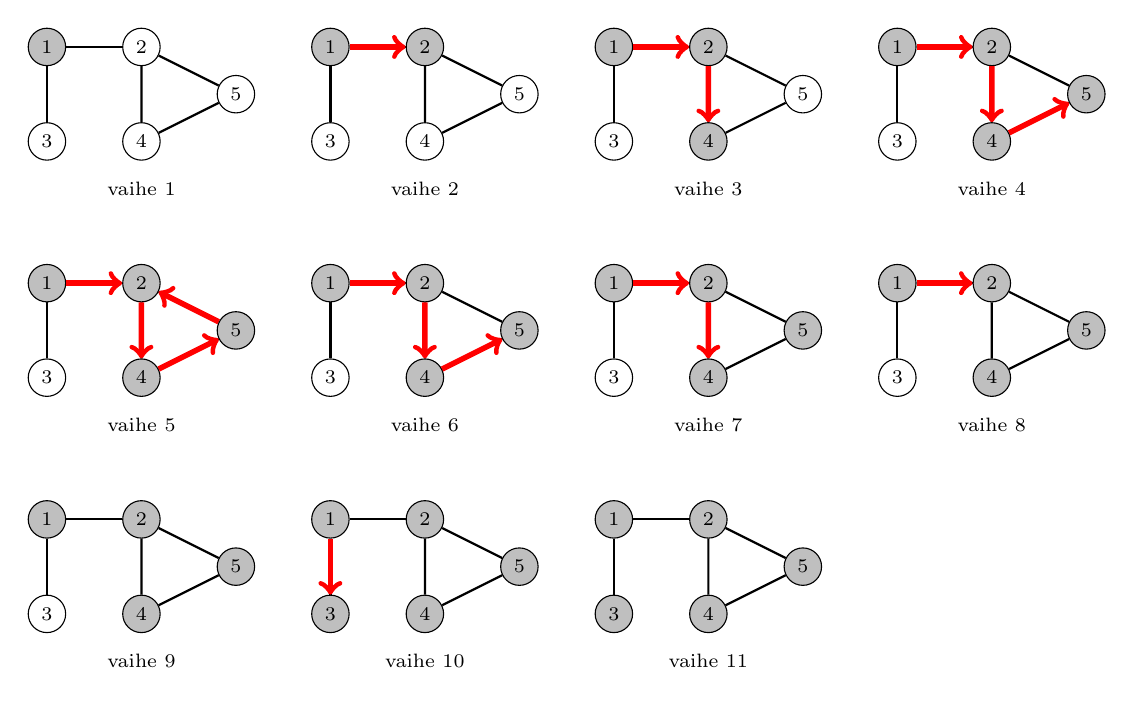
\begin{tikzpicture}[scale=0.6]
\scriptsize
\newcommand\verkko[6]{
\node[draw, circle, fill=#2] (1) at (0,0) {$1$};
\node[draw, circle, fill=#3] (2) at (2,0) {$2$};
\node[draw, circle, fill=#4] (3) at (0,-2) {$3$};
\node[draw, circle, fill=#5] (4) at (2,-2) {$4$};
\node[draw, circle, fill=#6] (5) at (4,-1) {$5$};
\path[draw,thick,-] (1) -- (2);
\path[draw,thick,-] (2) -- (5);
\path[draw,thick,-] (2) -- (4);
\path[draw,thick,-] (4) -- (5);
\path[draw,thick,-] (1) -- (3);
\node at (2,-3) {vaihe #1};
}
\begin{scope}
\verkko{1}{lightgray}{white}{white}{white}{white}
\end{scope}
\begin{scope}[xshift=6cm]
\verkko{2}{lightgray}{lightgray}{white}{white}{white}
\path[draw=red,thick,->,line width=2pt] (1) -- (2);
\end{scope}
\begin{scope}[xshift=12cm]
\verkko{3}{lightgray}{lightgray}{white}{lightgray}{white}
\path[draw=red,thick,->,line width=2pt] (1) -- (2);
\path[draw=red,thick,->,line width=2pt] (2) -- (4);
\end{scope}
\begin{scope}[xshift=18cm]
\verkko{4}{lightgray}{lightgray}{white}{lightgray}{lightgray}
\path[draw=red,thick,->,line width=2pt] (1) -- (2);
\path[draw=red,thick,->,line width=2pt] (2) -- (4);
\path[draw=red,thick,->,line width=2pt] (4) -- (5);
\end{scope}
\begin{scope}[yshift=-5cm]
\verkko{5}{lightgray}{lightgray}{white}{lightgray}{lightgray}
\path[draw=red,thick,->,line width=2pt] (1) -- (2);
\path[draw=red,thick,->,line width=2pt] (2) -- (4);
\path[draw=red,thick,->,line width=2pt] (4) -- (5);
\path[draw=red,thick,->,line width=2pt] (5) -- (2);
\end{scope}
\begin{scope}[yshift=-5cm,xshift=6cm]
\verkko{6}{lightgray}{lightgray}{white}{lightgray}{lightgray}
\path[draw=red,thick,->,line width=2pt] (1) -- (2);
\path[draw=red,thick,->,line width=2pt] (2) -- (4);
\path[draw=red,thick,->,line width=2pt] (4) -- (5);
\end{scope}
\begin{scope}[yshift=-5cm,xshift=12cm]
\verkko{7}{lightgray}{lightgray}{white}{lightgray}{lightgray}
\path[draw=red,thick,->,line width=2pt] (1) -- (2);
\path[draw=red,thick,->,line width=2pt] (2) -- (4);
\end{scope}
\begin{scope}[yshift=-5cm,xshift=18cm]
\verkko{8}{lightgray}{lightgray}{white}{lightgray}{lightgray}
\path[draw=red,thick,->,line width=2pt] (1) -- (2);
\end{scope}
\begin{scope}[yshift=-10cm]
\verkko{9}{lightgray}{lightgray}{white}{lightgray}{lightgray}
\end{scope}
\begin{scope}[yshift=-10cm,xshift=6cm]
\verkko{10}{lightgray}{lightgray}{lightgray}{lightgray}{lightgray}
\path[draw=red,thick,->,line width=2pt] (1) -- (3);
\end{scope}
\begin{scope}[yshift=-10cm,xshift=12cm]
\verkko{11}{lightgray}{lightgray}{lightgray}{lightgray}{lightgray}
\end{scope}
\end{tikzpicture}
\end{center}
\caption{Esimerkki syvyyshaun toiminnasta.}
\label{fig:syvhak}
\end{figure}

Kuvassa \ref{fig:syvhak} on esimerkki syvyyshaun toiminnasta.
Jokaisessa vaiheessa harmaat solmut ovat solmuja,
joissa haku on jo vieraillut.
Haku lähtee liikkeelle solmusta 1 ja etenee ensin
solmuihin 2, 4 ja 5.
Tämän jälkeen haku palaa takaisin solmuun 1
ja käy vielä solmussa 3.

\subsection{Algoritmin toteutus}

Syvyyshaku on mukavaa toteuttaa rekursiivisesti.
Tarvitsemme ensinnäkin taulukon, joka kertoo,
missä solmuissa olemme käyneet:

\begin{code}
boolean[] vierailtu = new boolean[n+1];
\end{code}

Tämän jälkeen voimme toteuttaa syvyyshaun näin:

\begin{code}
void syvyyshaku(int solmu) {
    if (vierailtu[solmu]) return;
    vierailtu[solmu] = true;
    for (Integer naapuri : verkko[solmu]) {
        syvyyshaku(naapuri);
    }
}
\end{code}

Syvyyshaku käynnistyy, kun kutsumme metodia
\texttt{syvyyshaku} parametrina lähtösolmu.
Jokaisella kutsulla metodi tarkistaa ensin,
olemmeko jo käyneet parametrina annetussa solmussa,
ja päättyy heti tässä tilanteessa.
Muuten metodi merkitsee, että olemme nyt käyneet solmussa
ja etenee rekursiivisesti kaikkiin solmun naapureihin.

Syvyyshaku vie aikaa $O(n+m)$, missä $n$ on solmujen määrä
ja $m$ on kaarten määrä,
koska käymme läpi kerran jokaisesta solmusta lähtevät kaaret.

\subsection{Sovelluksia}

\begin{figure}
\center
\begin{center}
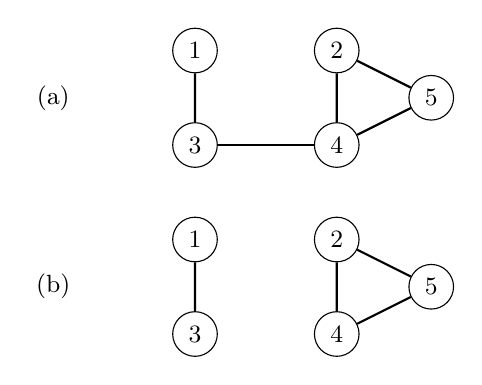
\begin{tikzpicture}[scale=0.6]
\small
\begin{scope}
\node[draw, circle] (1) at (1,3) {$1$};
\node[draw, circle] (2) at (4,3) {$2$};
\node[draw, circle] (3) at (1,1) {$3$};
\node[draw, circle] (4) at (4,1) {$4$};
\node[draw, circle] (5) at (6,2) {$5$};
\path[draw,thick,-] (1) -- (3);
\path[draw,thick,-] (3) -- (4);
\path[draw,thick,-] (2) -- (4);
\path[draw,thick,-] (2) -- (5);
\path[draw,thick,-] (4) -- (5);
\node at (-2,2) {(a)};
\end{scope}
\begin{scope}[yshift=-4cm]
\node[draw, circle] (1) at (1,3) {$1$};
\node[draw, circle] (2) at (4,3) {$2$};
\node[draw, circle] (3) at (1,1) {$3$};
\node[draw, circle] (4) at (4,1) {$4$};
\node[draw, circle] (5) at (6,2) {$5$};
\path[draw,thick,-] (1) -- (3);
\path[draw,thick,-] (2) -- (4);
\path[draw,thick,-] (2) -- (5);
\path[draw,thick,-] (4) -- (5);
\node at (-2,2) {(b)};
\end{scope}
\end{tikzpicture}
\end{center}
\caption{(a) Verkko on yhtenäinen. (b) Verkon yhtenäiset komponentit ovat $\{1,3\}$ ja $\{2,4,5\}$.}
\label{fig:veryht}
\end{figure}

Kun suoritamme verkossa syvyyshaun tietystä solmusta alkaen,
löydämme polut kaikkiin solmuihin, joihin kyseisestä
solmusta pääsee.
Esimerkiksi kuvan \ref{fig:syvhak} syvyyshaun aikana
olemme saaneet selville polut solmusta 1 kaikkiin muihin solmuihin.
Tässä tapauksessa esimerkiksi polku solmusta $1$ solmuun $5$ on
$1 \rightarrow 2 \rightarrow 4 \rightarrow 5$,
joka on löytynyt haun vaiheessa 4.

Sanomme, että verkko on \emph{yhtenäinen},
jos verkossa on polku minkä tahansa kahden solmun välillä.
Verkko on yhtenäinen tarkalleen silloin,
kun pääsemme \emph{mistä tahansa} solmusta
kaikkiin muihin solmuihin.
Niinpä voimme tarkastaa yhtenäisyyden suorittamalla
syvyyshaun mielivaltaisesta solmusta alkaen.
Esimerkiksi kuvan \ref{fig:veryht}(a) verkko on yhtenäinen,
koska solmusta 1 alkava syvyyshaku käy kaikissa solmuissa.

Jos verkko ei ole yhtenäinen, se jakautuu
yhtenäisiin \emph{komponentteihin},
joista jokainen sisältää solmut, jotka ovat yhteydessä
toisiinsa.
Esimerkiksi kuvan \ref{fig:veryht}(b) verkon
yhtenäiset komponentit ovat $\{1,3\}$ ja $\{2,4,5\}$.
Löydäm\-me verkon yhtenäiset komponentit
käymällä läpi kaikki verkon solmut ja aloittamalla
uuden syvyyshaun aina, kun emme ole käyneet solmussa aiemmin.
Jokainen syvyyshaku löytää yhden yhtenäisen komponentin.

\section{Leveyshaku}

\emph{Leveyshaku} on algoritmi, joka selvittää \emph{lyhimmän} polun
lähtösolmusta kaikkiin solmuihin, jotka ovat saavutettavissa siitä.
Lyhin polku tarkoittaa polkua, jossa on mahdollisimman vähän kaaria.
Käsittelemme solmut kerroksittain lähtösolmusta alkaen
siinä järjestyksessä kuin olemme löytäneet ne.
Jokaisen solmun kohdalla käymme läpi kaikki siitä lähtevät kaaret.

\begin{figure}
\center
\begin{center}
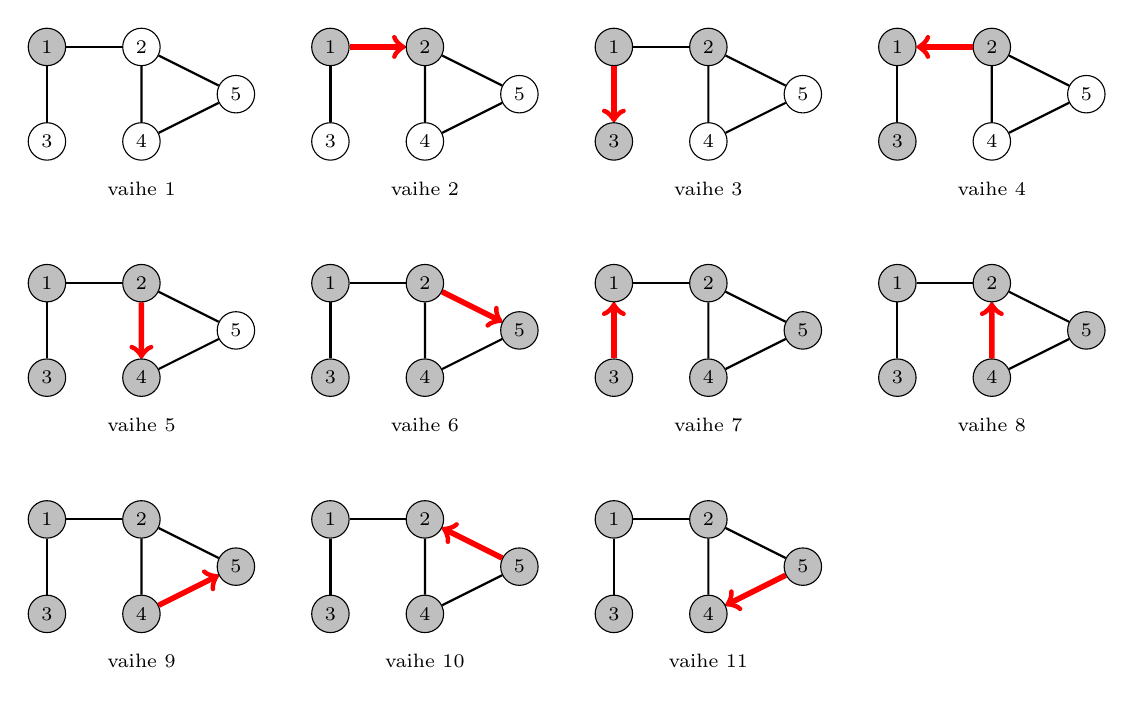
\begin{tikzpicture}[scale=0.6]
\scriptsize
\newcommand\verkko[6]{
\node[draw, circle, fill=#2] (1) at (0,0) {$1$};
\node[draw, circle, fill=#3] (2) at (2,0) {$2$};
\node[draw, circle, fill=#4] (3) at (0,-2) {$3$};
\node[draw, circle, fill=#5] (4) at (2,-2) {$4$};
\node[draw, circle, fill=#6] (5) at (4,-1) {$5$};
\path[draw,thick,-] (1) -- (2);
\path[draw,thick,-] (2) -- (5);
\path[draw,thick,-] (2) -- (4);
\path[draw,thick,-] (4) -- (5);
\path[draw,thick,-] (1) -- (3);
\node at (2,-3) {vaihe #1};
}
\begin{scope}
\verkko{1}{lightgray}{white}{white}{white}{white}
\end{scope}
\begin{scope}[xshift=6cm]
\verkko{2}{lightgray}{lightgray}{white}{white}{white}
\path[draw=red,thick,->,line width=2pt] (1) -- (2);
\end{scope}
\begin{scope}[xshift=12cm]
\verkko{3}{lightgray}{lightgray}{lightgray}{white}{white}
\path[draw=red,thick,->,line width=2pt] (1) -- (3);
\end{scope}
\begin{scope}[xshift=18cm]
\verkko{4}{lightgray}{lightgray}{lightgray}{white}{white}
\path[draw=red,thick,->,line width=2pt] (2) -- (1);
\end{scope}
\begin{scope}[yshift=-5cm,xshift=0cm]
\verkko{5}{lightgray}{lightgray}{lightgray}{lightgray}{white}
\path[draw=red,thick,->,line width=2pt] (2) -- (4);
\end{scope}
\begin{scope}[yshift=-5cm,xshift=6cm]
\verkko{6}{lightgray}{lightgray}{lightgray}{lightgray}{lightgray}
\path[draw=red,thick,->,line width=2pt] (2) -- (5);
\end{scope}
\begin{scope}[yshift=-5cm,xshift=12cm]
\verkko{7}{lightgray}{lightgray}{lightgray}{lightgray}{lightgray}
\path[draw=red,thick,->,line width=2pt] (3) -- (1);
\end{scope}
\begin{scope}[yshift=-5cm,xshift=18cm]
\verkko{8}{lightgray}{lightgray}{lightgray}{lightgray}{lightgray}
\path[draw=red,thick,->,line width=2pt] (4) -- (2);
\end{scope}
\begin{scope}[yshift=-10cm,xshift=0cm]
\verkko{9}{lightgray}{lightgray}{lightgray}{lightgray}{lightgray}
\path[draw=red,thick,->,line width=2pt] (4) -- (5);
\end{scope}
\begin{scope}[yshift=-10cm,xshift=6cm]
\verkko{10}{lightgray}{lightgray}{lightgray}{lightgray}{lightgray}
\path[draw=red,thick,->,line width=2pt] (5) -- (2);
\end{scope}
\begin{scope}[yshift=-10cm,xshift=12cm]
\verkko{11}{lightgray}{lightgray}{lightgray}{lightgray}{lightgray}
\path[draw=red,thick,->,line width=2pt] (5) -- (4);
\end{scope}
\end{tikzpicture}
\end{center}
\caption{Esimerkki leveyshaun toiminnasta.}
\label{fig:levhak}
\end{figure}

Kuvassa \ref{fig:levhak} on esimerkki leveyshaun toiminnasta,
kun etsimme polkuja solmusta 1 aloittaen.
Käsittelemme ensin solmun 1, josta pääsemme uusiin solmuihin 2 ja 3.
Sitten käsittelemme solmun 2, josta pääsemme uusiin solmuihin 4 ja 5.
Lopuksi käsittelemme vielä solmut 3, 4 ja 5,
joista emme kuitenkaan pääse enää uusiin solmuihin.

\subsection{Algoritmin toteutus}

Leveyshaku on vaikeampi toteuttaa kuin syvyyshaku,
koska meidän täytyy pystyä edistämään hakua vuorotellen verkon eri puolilta.
Tätä varten luomme \emph{jonon}, joka sisältää läpikäyntiä odottavia solmuja.
Valitsemme aina seuraavaksi käsiteltävän solmun jonon alusta,
ja lisämme uudet vieraillut solmut jonon loppuun.
Voimme luoda jonon näin:

\begin{code}
ArrayDeque<Integer> jono = new ArrayDeque<>();
\end{code}

Lisäksi määrittelemme syvyyshaun tapaan taulukon, jossa pidämme kirjaa,
missä solmuissa olemme käyneet:

\begin{code}
boolean[] vierailtu = new boolean[n+1];
\end{code}

Nyt voimme toteuttaa leveyshaun seuraavasti solmusta \texttt{alku} lähtien:

\begin{code}
vierailtu[alku] = true;
jono.addLast(alku);
while (jono.size() > 0) {
    int solmu = jono.pollFirst();
    for (int naapuri : verkko[solmu]) {
        if (vierailtu[naapuri]) continue;
        vierailtu[naapuri] = true;
        jono.addLast(naapuri);
    }
}
\end{code}

Koodi merkitsee aluksi, että olemme käyneet lähtösolmussa
sekä lisää lähtösolmun jonoon.
Tämän jälkeen joka askeleella haku valitsee
jonon ensimmäisen solmun ja tarkastaa siitä lähtevät kaaret.
Jos pääsemme uuteen solmuun, merkitsemme uuden solmun
vierailluksi ja lisäämme sen jonoon.
Haku jatkuu niin kauan kuin jonossa on solmuja.

Syvyyshaun tavoin leveyshaku vie aikaa $O(n+m)$,
koska käymme läpi kerran jokaisesta solmusta lähtevät kaaret.

\subsection{Polkujen etsiminen}

Vaikka leveyshakua voi käyttää yleisalgoritmina verkon läpikäyntiin,
yleensä tavoitteena on nimenomaan löytää lyhimmät polut lähtösolmusta
muihin solmuihin. Tätä varten määrittelemme kaksi uutta taulukkoa:

\begin{code}
int[] etaisyys = new int[n+1];
int[] aiempi = new int[n+1];
\end{code}

Taulukko \texttt{etaisyys} kertoo, mikä on etäisyys
(eli lyhimmän polun pituus) lähtösolmusta solmuun,
ja taulukko \texttt{aiempi} viittaa edelliseen solmuun lyhimmällä polulla.
Näiden taulukoiden avulla voimme leveyshaun jälkeen muodostaa
lyhimmän polun lähtösolmusta mihin tahansa solmuun.
Päivitäm\-me taulukoita seuraavasti haun aikana:

\begin{code}
vierailtu[alku] = true;
etaisyys[alku] = 0;
aiempi[alku] = 0;
jono.addLast(alku);
while (jono.size() > 0) {
    int solmu = jono.pollFirst();
    for (int naapuri : verkko[solmu]) {
        if (vierailtu[naapuri]) continue;
        vierailtu[naapuri] = true;
        etaisyys[naapuri] = etaisyys[solmu]+1;
        aiempi[naapuri] = solmu;
        jono.addLast(naapuri);
    }
}
\end{code}

Haun alussa merkitsemme, että etäisyys lähtösolmuun on 0
ja sillä ei ole edellistä solmua.
Sitten kun löydämme uuden solmun, päivitämme sen etäisyyden
ja edellisen solmun polulla.

Nyt leveyshaun jälkeen lyhimmän polun pituus lähtösolmusta
solmuun $x$ on $\texttt{etaisyys}[x]$ ja voimme käydä läpi polulla
olevat solmut seuraavasti (käänteisessä järjestyksessä):

\begin{code}
while (x != 0) {
    System.out.println(x);
    x = aiempi[x];
}
\end{code}

\section{Esimerkki: Labyrintti}

Olemme labyrintissa ja haluamme päästä ruudusta $A$ ruutuun $B$.
Joka askeleella voimme siirtyä yhden ruudun verran ylöspäin, alaspäin,
vasemmalle tai oikealle.
Pystymmekö pääsemään ruudusta $A$ ruutuun $B$, ja jos pystymme, niin
mikä on lyhin mahdollinen reitti?
Esimerkiksi kuvassa \ref{fig:labrei}(a) lyhin reitti
ruudusta $A$ ruutuun $B$ muodostuu 9 askeleesta.

\begin{figure}
\center
\begin{center}
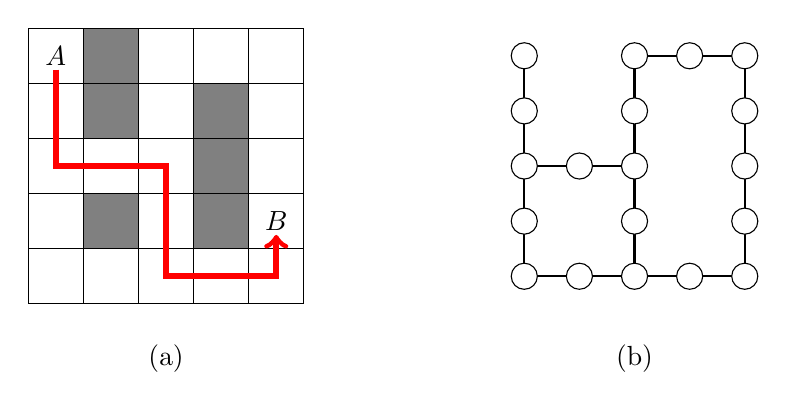
\begin{tikzpicture}[scale=0.7]
\begin{scope}
\draw[fill=gray] (1,1) rectangle (2,2);
\draw[fill=gray] (1,3) rectangle (2,4);
\draw[fill=gray] (1,4) rectangle (2,5);
\draw[fill=gray] (3,1) rectangle (4,2);
\draw[fill=gray] (3,2) rectangle (4,3);
\draw[fill=gray] (3,3) rectangle (4,4);
\draw (0,0) grid (5,5);
\draw[->,thick,red,line width=2pt] (0.5,4.25) -- (0.5,2.5) -- (2.5,2.5) -- (2.5,0.5) -- (4.5,0.5) -- (4.5,1.25);
\node at (0.5,4.5) {$A$};
\node at (4.5,1.5) {$B$};
\node at (2.5,-1) {(a)};
\end{scope}
\begin{scope}[xshift=9cm,yshift=0.5cm]
\foreach \x in {0,1,2,3} \path[draw,thick,-] (0,\x) -- (0,\x+1);
\foreach \x in {0,1,2,3} \path[draw,thick,-] (2,\x) -- (2,\x+1);
\foreach \x in {0,1,2,3} \path[draw,thick,-] (4,\x) -- (4,\x+1);
\foreach \x in {0,1,2,3} \path[draw,thick,-] (\x,0) -- (\x+1,0);
\foreach \x in {0,1} \path[draw,thick,-] (\x,2) -- (\x+1,2);
\foreach \x in {2,3} \path[draw,thick,-] (\x,4) -- (\x+1,4);
\foreach \x in {0,1,2,3,4} \node[draw, circle, fill=white] at (0,\x) {};
\foreach \x in {0,2} \node[draw, circle, fill=white] at (1,\x) {};
\foreach \x in {0,1,2,3,4} \node[draw, circle, fill=white] at (2,\x) {};
\foreach \x in {0,4} \node[draw, circle, fill=white] at (3,\x) {};
\foreach \x in {0,1,2,3,4} \node[draw, circle, fill=white] at (4,\x) {};
\node at (2,-1.5) {(b)};
\end{scope}
\end{tikzpicture}
\end{center}
\caption{(a) Lyhin reitti labyrintissa ruudusta $A$ ruutuun $B$. (b)
Labyrintin esittäminen verkkona.}
\label{fig:labrei}
\end{figure}

Voimme esittää ongelman verkkona niin,
että jokainen labyrintin ruutu on yksi verkon solmuista,
ja kahden solmun välillä on kaari,
jos vastaavat ruudut ovat vierekkäin labyrintissa.
Kuva \ref{fig:labrei}(b) näyttää esimerkkilabyrinttimme verkkona.
Nyt ruudusta $A$ on reitti ruutuun $B$ tarkalleen silloin,
kun vastaavat verkon solmut kuuluvat samaan komponenttiin,
minkä voimme tarkastaa syvyyshaulla.
Lyhin reitti ruudusta $A$ ruutuun $B$ löytyy puolestaan leveyshaulla,
joka lähtee liikkeelle ruudusta $A$.

Huomaa, että meidän ei tarvitse erikseen muuttaa labyrinttia
verkoksi, vaan voimme toteuttaa haut \emph{implisiittiseen} verkkoon.
Tämä tarkoittaa, että teemme haun labyrinttiin sen omassa
esitysmuodossa. Käytännössä labyrintti on kätevää tallentaa kaksiulotteisena
taulukkona, joka ilmaisee, mitkä ruudut ovat lattiaa ja seinää.
Tällöin voimme toteuttaa esimerkiksi syvyyshaun seuraavan tyylisesti:

\begin{code}
void syvyyshaku(int y, int x) {
    if (y < 0 || x < 0 || y >= n || x >= n) return;
    if (seina[y][x] || vierailtu[y][x]) return;
    vierailtu[y][x] = true;
    syvyyshaku(y+1,x);
    syvyyshaku(y-1,x);
    syvyyshaku(y,x+1);
    syvyyshaku(y,x-1);
}
\end{code}